\documentclass[12pt]{article}

% French
\usepackage[utf8]{inputenc}
\usepackage[T1]{fontenc}
\usepackage[french]{babel}

\usepackage{hyperref}
\usepackage{pdfpages}
\usepackage{float}
\usepackage{geometry}
\usepackage{tikz}
\usepackage{eurosym}

\usepackage{multirow}
\usepackage{datetime}

\usepackage{titlesec}

\titleformat*{\section}{\LARGE\bfseries}
\titleformat*{\subsection}{\Large\bfseries}
\titleformat*{\subsubsection}{\large\bfseries}
\titleformat*{\paragraph}{\large\bfseries}
\titleformat*{\subparagraph}{\large\bfseries}


\geometry{margin=2.5cm}

\definecolor{darkgreen}{RGB}{0,130,0}
\definecolor{darkblue}{RGB}{0,0,130}

\newcommand{\gameName}{\textit{Lands of Azerith}}
\newcommand{\companyName}{Stonks Industries}
% \newcommand{\progressbar}[1]{
%     \begin{tikzpicture}
%         \fill[black!30] (0,0) rectangle (#1/100*2cm, 0.2);
%         \draw (0,0) rectangle (2cm, 0.2);
%     \end{tikzpicture}
%     \small{#1\%}
% }


\title{
    Rapport de la première Soutenance \\
    \textbf{\gameName} \\
    \vspace{0.5cm}
    
\includegraphics[width=5cm]{0.format/logo.png}
    \vspace{4.2cm}
}
\author{
    Ayemane Bouarbi \\
    \texttt{ayemane.bouarbi@epita.fr}
    \vspace{0.5cm}\and
    Alexandre Cölsch \\
    \texttt{alexandre.colsch@epita.fr}
    \vspace{0.5cm}\and
    Michaël Museux \\
    \texttt{michael.museux@epita.fr}
    \vspace{0.5cm}\and
    Martin Pasquier \\
    \texttt{martin.pasquier@epita.fr}
}

\date{
    \vspace{1.5cm}
    \textbf{\companyName} \\
    \vspace{0.3cm}
    \textbf{EPITA} \\
    \vspace{1.5cm}
    \today
}

\begin{document}

\begin{titlepage}
    \maketitle
    \thispagestyle{empty} % Remove page number from title page
\end{titlepage}

\newpage
\thispagestyle{empty}
\mbox{}

\newpage
\tableofcontents

\newpage
\section{Introduction}
% Written by multiple authors

À mi-parcours de la réalisation de notre jeu vidéo \gameName, il est temps de faire un bilan de ce que nous avons accompli jusqu'à présent.
L'ojectif de ce rapport est de faire un point sur l'avancement du projet, d'en tirer des conclusions et de définir les objectifs à atteindre pour la suite.
\\

L'équipe de cinq personnes à l'origine de ce projet a travaillé pendant plusieurs mois, pendant lesquels elle a su faire face aux difficultés rencontrées. 
Nous avons appris à travailler ensemble, à nous organiser, à gérer notre temps et à prendre des décisions. 
\\

La première partie de ce rapport sera consacrée au bilan de la réalisation du projet dans sa globalité. 
Nous y aborderons l'avancement du site web et les changements d'organisation que nous avons effectués, ainsi que les difficultés associées.
\\

La deuxième partie sera consacrée à l'analyse du jeu. 
Avec un point de vue technique, nous y aborderons les choix que nous avons fait, les fonctionnalités déjà implémentées et celles que nous n'avons pas pu terminer.
\\




\newpage
\section{Le projet}

\subsection{Changements depuis la dernière soutenance}
% TODO Write about the changes in the project

Certains changements sont survenus dans le projet depuis la dernière rédaction du cahier des charges. Certains portent à l'organisations du travail, d'autres sont techniques. 

Le nom du jeu a été changé, il s'appelle maintenant "\gameName". Ce changement a été motivé par un changement d'inspiration pour le jeu, et par la volonté de se démarquer des autres jeux. Le cahier des charges a été mis à jour pour refléter ce changement il y a plusieurs mois maintenant.

Tout d'abord, le départ d'un de nos membres a nécessité une réorganisation de l'équipe. En effet Mohamed Aziz a quitté le projet pour des raisons personnelles. Cela a nécessité une réorganisation de l'équipe, et une adaptation de l'organisation du travail.

Ses taches ont été réparties entre les autres membres de l'équipe pour ne pas retarder le projet. Cela a entraîné un ralentissement des taches de développement, mais n'a pas retardé le projet pour autant.

Cela fait partie des difficultés que nous avons rencontrées, mais nous avons su les surmonter. Cela a permis à l'équipe de se renforcer et de mieux comprendre les taches des autres membres. La redondance des taches a donc été intensifiée pour mieux assurer l'avenir du jeu.

\subsection{Site web}
% Written by Martin Pasquier (Marty42780)

Le site web est une tache secondaire du projet, mais il est tout de même important pour la communication et la promotion du jeu.
Il est essentiel pour permettre aux joueurs de découvrir le jeu, de suivre son développement et de le télécharger.
C'est l'outils central de la partie communication du projet, et il est donc important de le maintenir à jour dse dernières informations sur le jeu.
\\

\subsubsection*{\hspace*{0.6cm}Avancement du site web}


Sa phase de développement est finie, il est maintenant en attente de contenu du jeu et d'être publié.
En effet du contenu du jeu tel que des images ou des vidéos de gameplay sont nécessaires pour le site web, et ces éléments ne sont pas encore prêts. En attente de ces éléments, le site web utilise des images et des vidéos de démonstration appelés "\textit{placeholders}".


\begin{figure}[H]
    \centering
    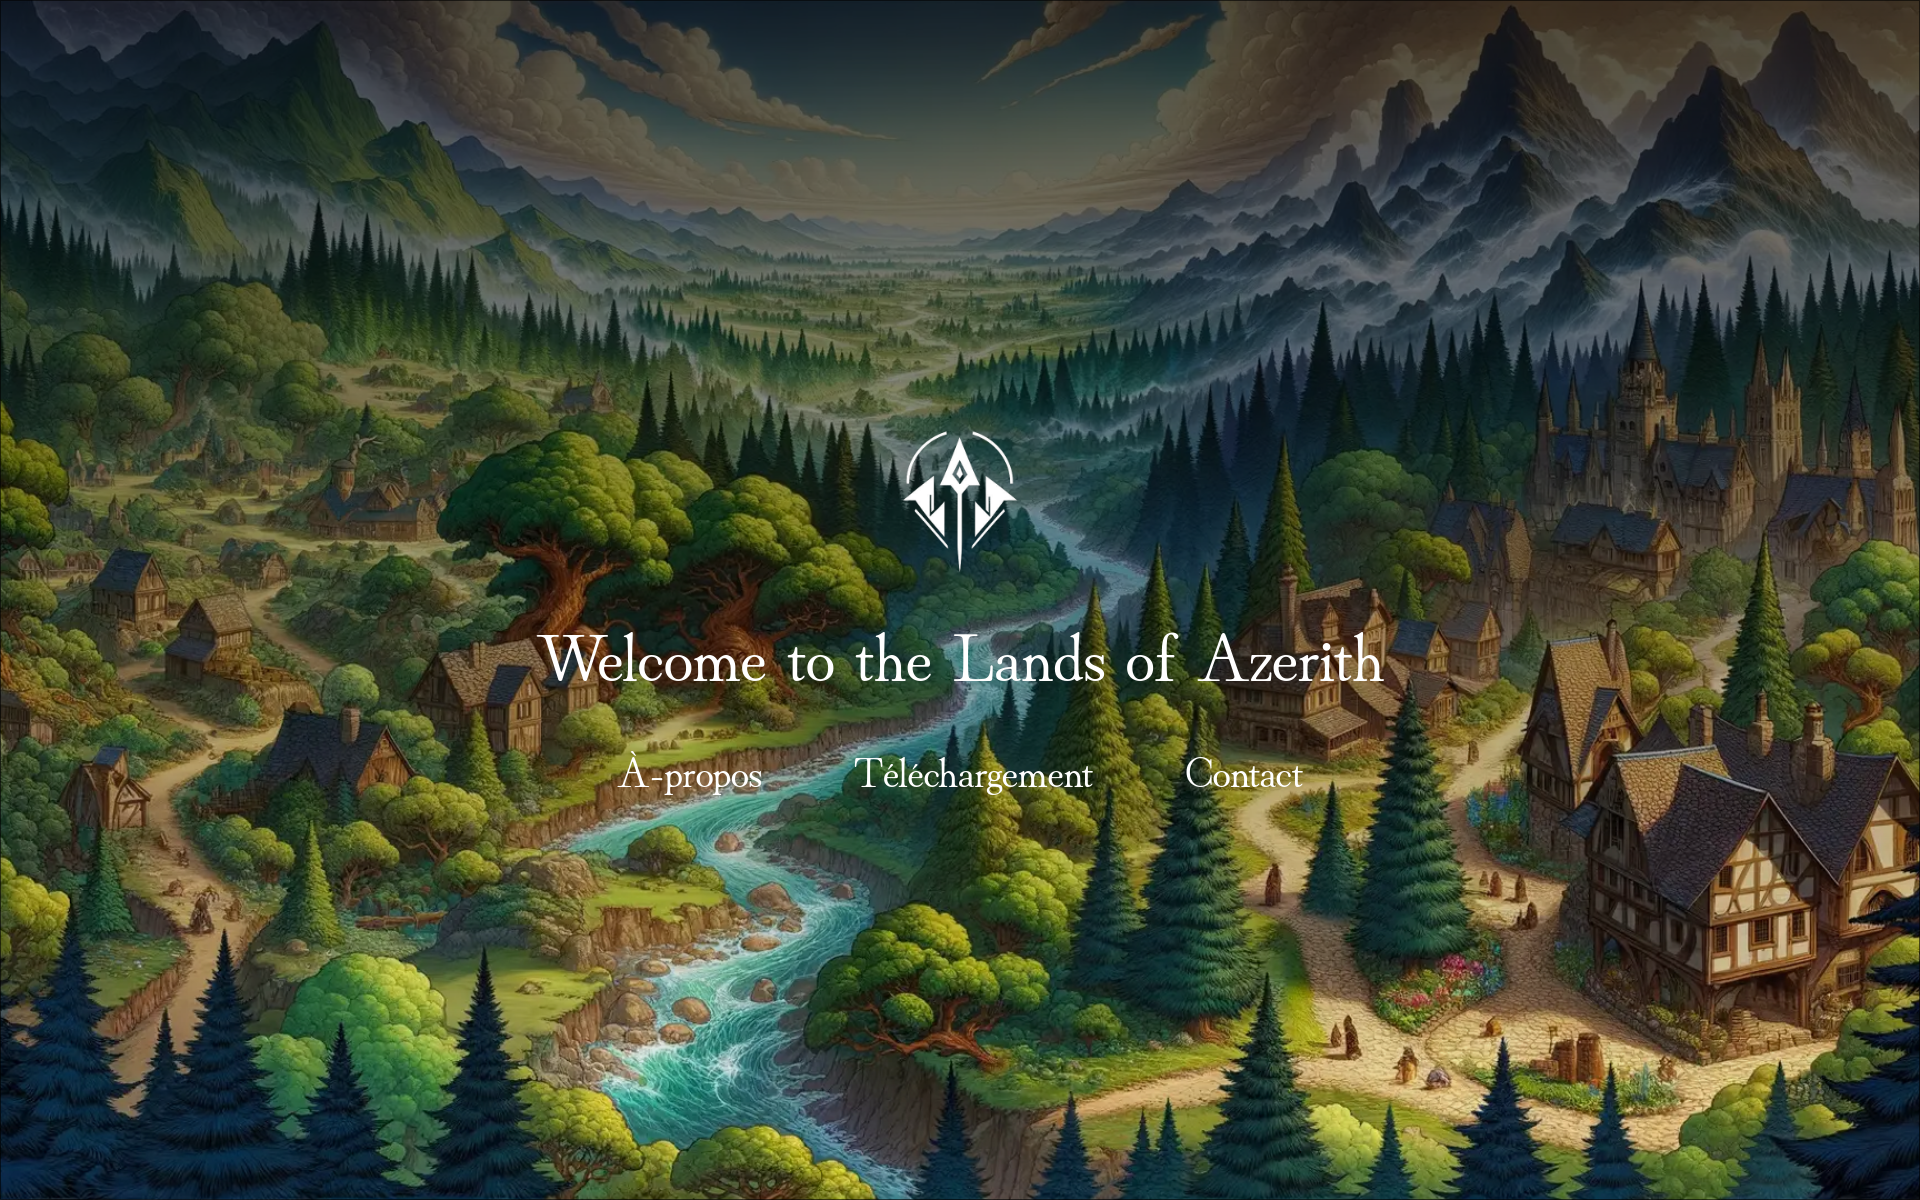
\includegraphics[width=0.8\textwidth]{2.game/assets/website1.png}
    \caption{Page d'accueil du site web, elle représente bien la simplicité voulu pour le site web.}
    \label{fig:website1}
\end{figure}

Comme le montre la \ref*{fig:website1}, le site web est simple et épuré. 
Il est composé d'une seule page, laissant l'utilisateur scroller pour découvrir les différentes sections.
Elle possède un menu de navigation qui permet de se rendre directement aux sections les plus importantes du site web, et un pied de page avec des liens vers les réseaux sociaux et le dépôt de code source du jeu.
\\

Les différentes sections sont les suivantes :

- "À propos", cette partie présente le jeu, son style et le concept associé

- "Téléchargement", pour télécharger le jeu pour les différentes plateformes

- "Contact", pour contacter l'équipe de développement en redirigeant l'utilisateur vers une adresse mail ou le dépôt GitHub du projet


\subsubsection*{\hspace*{0.6cm}Technologies utilisées}

Le site possède son propre dépôt de code source sur \textit{GitHub} à l'adresse \url{https://github.com/StonksIndustries/Azerith_Website}. 

Nous avons utilisé l'éditeur de code VSCode pour développer le site web car il offre de nombreux outils très outils pour cela. On peut citer l'intégration avec \textit{GitHub}, les extensions pour le développement web, et les outils de débogage intégrés.
\\

Le site web est développé en HTML, SCSS et JS, et est compilé avec Parcel. 
Leur choix a été motivé par leur simplicité et leur popularité, qui permettent de trouver facilement de l'aide en cas de problème. 
Parcel permet de compiler le site web sans aucune configuration et une très bonne optimisation des fichiers. 
Le \textit{SCSS}, remplace le \textit{CSS} pour permettre une meilleure organisation du code et une meilleure maintenabilité. 
Le JS est utilisé pour les animations et les interactions avec le visiteur.
\\

Il sera automatiquement compilé et publié grâce aux outils \textit{GitHub Actions} et \textit{GitHub Pages}. 
L'usage de ces outils permet de simplifier la publication du site web, et de le mettre à jour automatiquement à chaque modification du code source. 
Chaque nouvelle versions envoyés par un développeur est automatiquement compilée et publiée sur le site web si aucune erreur n'est détectée.

Voici le lien du site web : \url{https://stonksindustries.github.io/Azerith_Website/dist}

\subsubsection*{\hspace*{0.6cm}Objectifs futurs}

Une fois les phases de développement et de publication terminées, le site web sera mis à jour régulièrement avec les dernières informations sur le jeu. Cela comprend les étapes de développement, les nouvelles fonctionnalités et les correctifs de bugs.
\\

Des améliorations sont cependant possibles, on peut lister les suivantes:

- Compatibilité avec les appareils mobiles ("\textit{responsive design}")

- Écran de chargement et animations

- Plus d'interactivité avec le visiteur (formulaire de contact, \textit{sliders} interactifs, etc.)



\subsection{Cahier des Charges Technique}
% This file CAN NOT be compiled on its own
% It is included by ../Book_of_Specifications.tex


% TODO Update the technical book

Les deux prochaines pages sont dédiées au cahier des charges technique.
Ce document détaille les contraintes et les caractéristiques techniques nécessaires pour répondre aux besoins du projet.
Il synthétise toutes les réponses aux questions techniques que l'on peut se poser sur le projet.
\\

Le cahier des charges technique est divisé en deux parties.
La première partie détaille les spécificités du jeu et les choix techniques qui ont été réalisés. 
La deuxième partie donne des informations sur la repartition des tâches et leur avancement.
\\

Des changements ont été apportés au cahier des charges technique depuis sa dernière version.
Le nom du jeu a été modifié, le départ de Mohamed Aziz a été pris en compte, et des changements ont été apportés au diagramme de Gantt pour refléter l'avancé du projet.


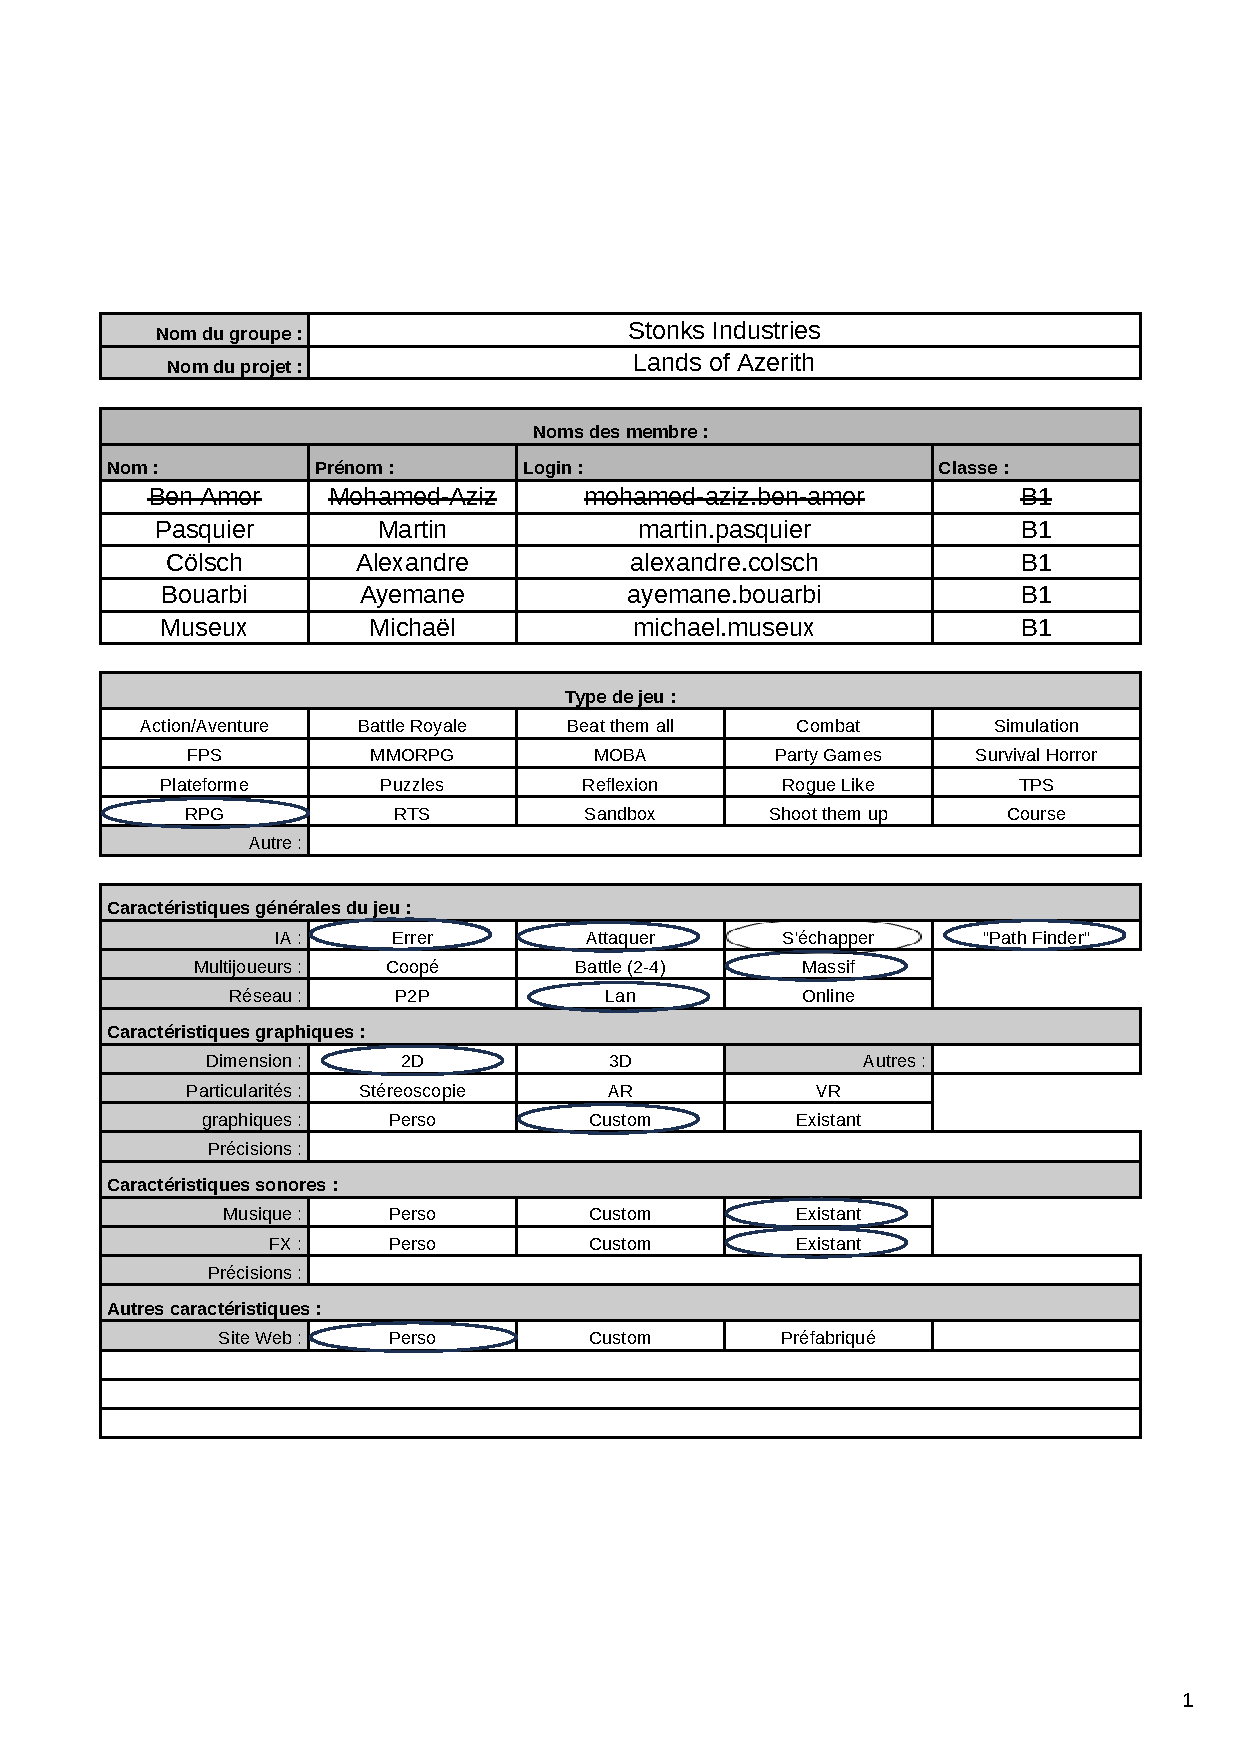
\includepdf[pages=1]{1.project/technical_book/page-1.pdf}

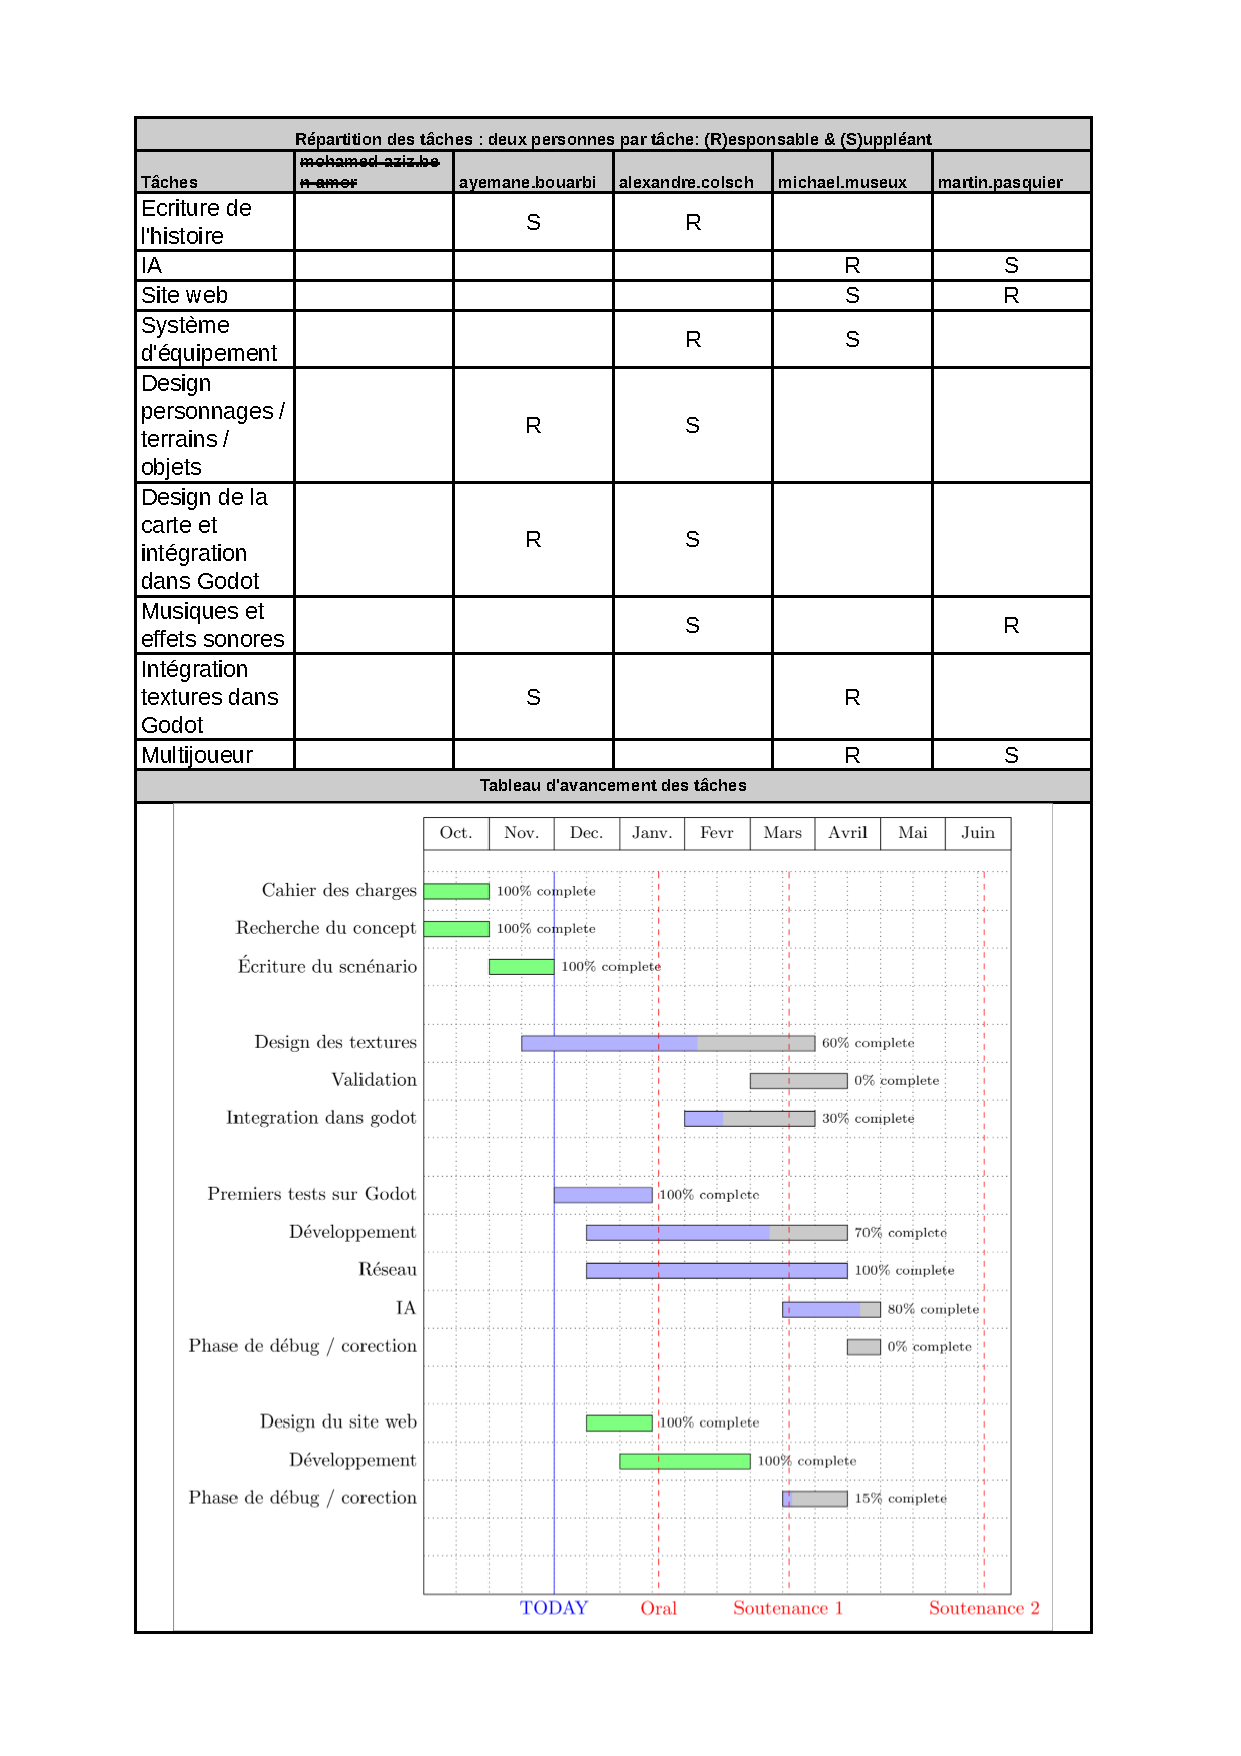
\includepdf[pages=1]{1.project/technical_book/page-2.pdf}


\newpage
\section{Le jeu}

\subsection{IA, Mécaniques de gameplay}
% Written by Michaël Museux

\subsubsection*{Le Multijoueur}

Pour pouvoir organiser une partie multijoueur, nous avons décidé d'utiliser l'API intégrée à Godot.
Pour cela, il nous faut un serveur, ici l'hôte, ainsi que les joueurs qui rejoignent sa partie appelés les clients,
En premier temps, l'hôte doit choisir quel port il souhaite utiliser pour sa partie, puis les joueurs doivent accéder à l'adresse de l'hôte, ainsi que le port précédemment choisi (cf Figure \ref{fig:gameplay1} et \ref*{fig:gameplay2}).

\begin{figure}[H]
    \centering
    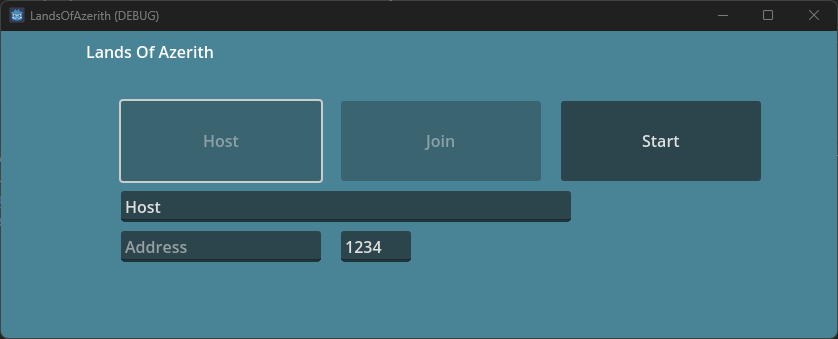
\includegraphics[width=0.8\textwidth]{2.game/assets/gameplay1.png}
    \caption{L'hôte clique sur "Host" et choisi le port 1234}
    \label{fig:gameplay1}
\end{figure}

\begin{figure}[H]
    \centering
    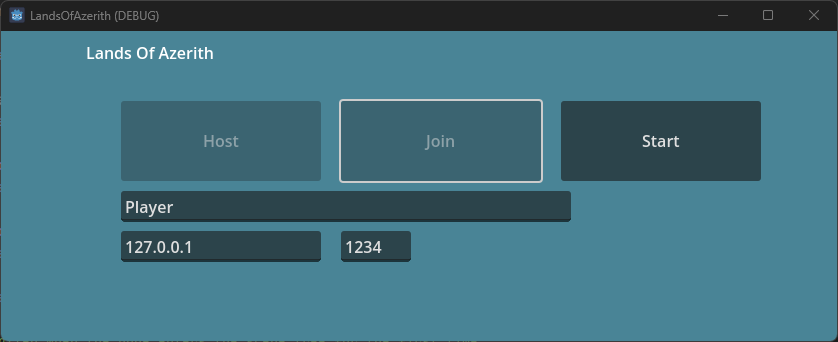
\includegraphics[width=0.8\textwidth]{2.game/assets/gameplay2.png}
    \caption{Le client clique sur "Join" et choisi le port 1234 à l'adresse 127.0.0.1.}
    \label{fig:gameplay2}
\end{figure}

Il est possible de jouer avec un nombre infini de joueurs, mais nous avons établi un maximum de 8, limite que nous utiliserons lors de la conception du reste du jeu.
\\

Maintenant que la connexion est établie entre les différents joueurs, il nous faut synchroniser les informations entre l'hosts et les différents clients, tout en faisant attention à ne pas trop partager d'informations inutiles, afin de limiter l'utilisation de bande passante.
Par exemple, la synchronisation des positions de chacun entre tous les joueurs est importante, mais la position de la caméra de chaque joueur n'est nécessaire qu'en local (c.f. Figures \ref*{fig:gameplay3} et \ref*{fig:gameplay4}).

\begin{figure}[H]
    \centering
    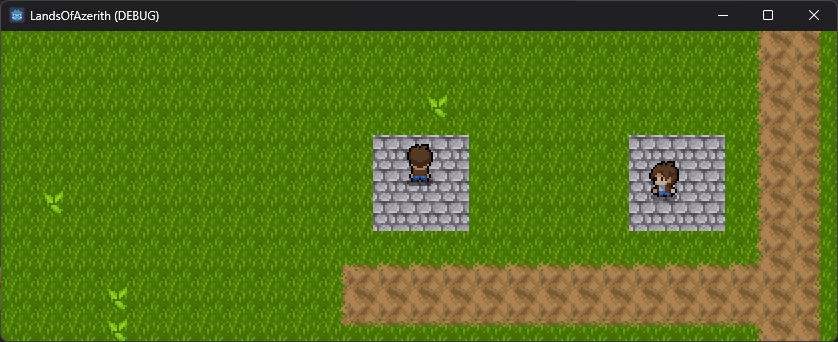
\includegraphics[width=0.8\textwidth]{2.game/assets/gameplay3.png}
    \caption{Le joueur 1 regarde vers le haut sur le carré de gauche avec sa caméra centré sur lui, le joueur 2 est à droite.}
    \label{fig:gameplay3}
\end{figure}

\begin{figure}[H]
    \centering
    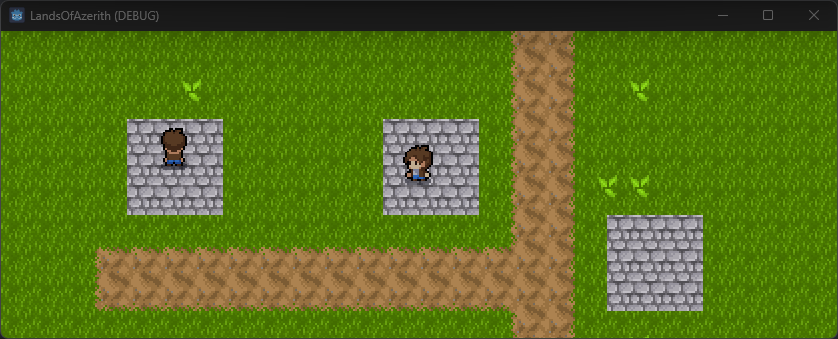
\includegraphics[width=0.8\textwidth]{2.game/assets/gameplay4.png}
    \caption{Le joueur 2 regarde vers la gauche sur le carré de droite avec sa caméra centré sur lui, le joueur 1 est à gauche.}
    \label{fig:gameplay4}
\end{figure}


\subsubsection*{Déplacement et comportement des PNJ}

Au cours des aventures de nos joueurs, ceux-ci rencontreront des monstres et animaux, passifs ou agressifs.
Il nous faut donc implémenter ces différents comportements.
Pour commencer, chaque PNJ est dans l'état “\textit{Wander}”, c'est-à-dire qu'il va soit trouver un endroit aléatoire où aller, soit rester sur place (c.f. Figure 5)

\begin{figure}[H]
    \centering
    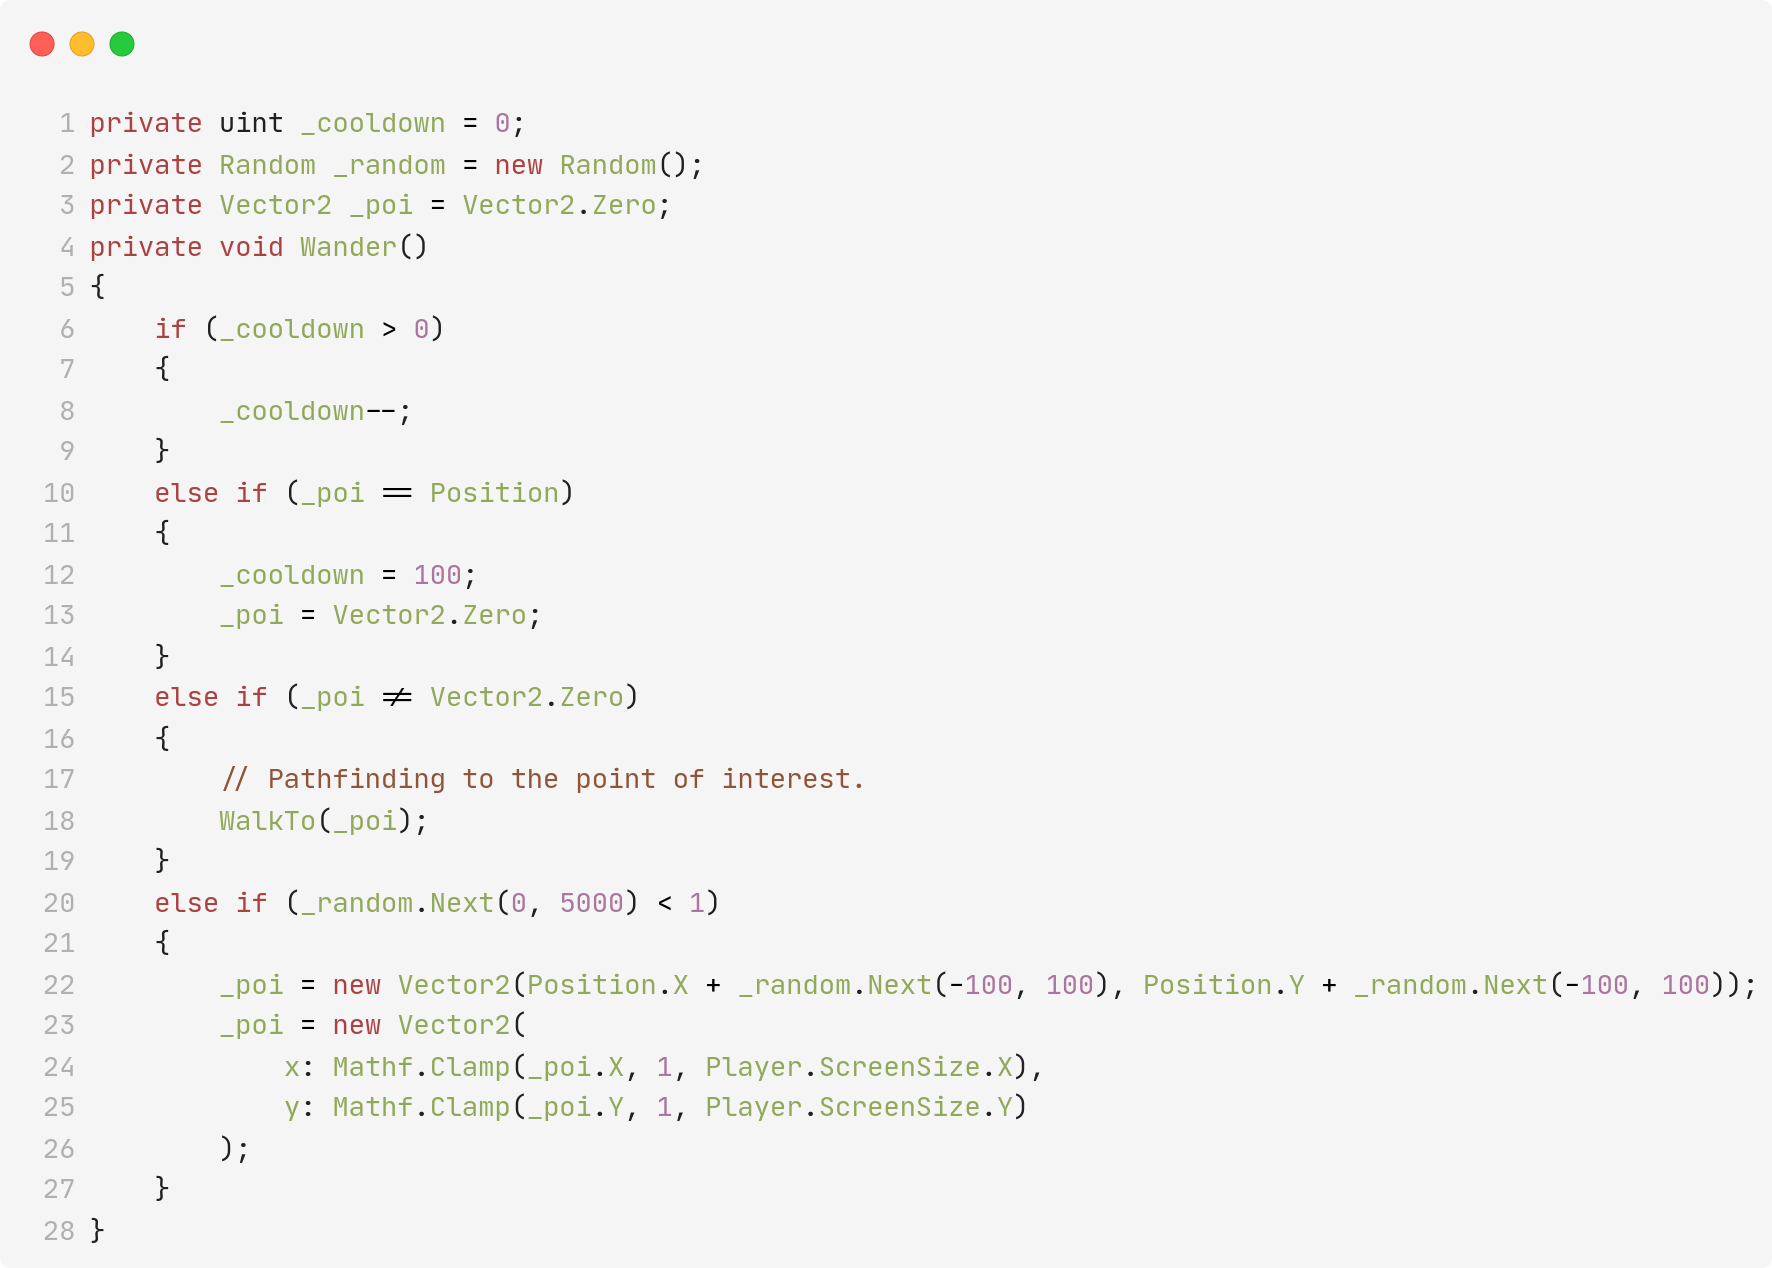
\includegraphics[width=1.0\textwidth]{2.game/assets/gameplay5.png}
    \caption{Code C\# décrivant le comportement durant l'état “\textit{Wander}”}
    \label{fig:gameplay5}
\end{figure}

Ensuite, le comportement d'une créature va brancher en quatre catégories distinctes :

- Le PNJ Agressif va attaquer le joueur lorsqu'il est à proximité

- Le PNJ Neutre ne va pas réagir au joueur lorsqu'il est à proximité, mais va répondre à ses attaques

- Le PNJ Passif ne va pas réagir au joueur lorsqu'il est à proximité, mais va fuir s'il est attaqué

- Le PNJ Peureux va fuir lorsqu'il est à proximité du joueur.
\\

\begin{figure}[H]
    \centering
    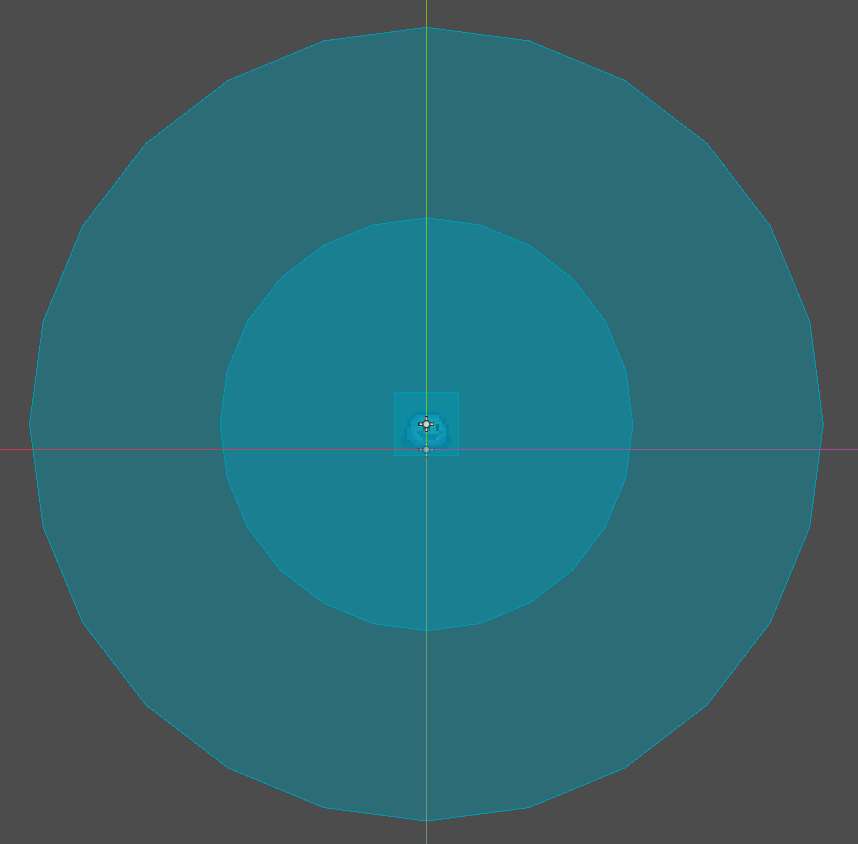
\includegraphics[width=0.8\textwidth]{2.game/assets/gameplay6.png}
    \caption{PNJ Agressif, avec ses zones d'\textit{aggro} et de \textit{déaggro}}
    \label{fig:gameplay6}
\end{figure}

Pour la détection du joueur, nous allons utiliser la fonctionnalité des signaux de Godot, et initier deux zones de détection circulaire autour de chaque monstre.
La première servira à détecter lorsque le joueur rentre dans cette zone (zone d'aggro), et la deuxième, un peu plus grande, qui détectera la sortie du joueur de cette zone (zone de déaggro), et qui repassera le PNJ dans l'état \textit{Wander}.
On ne veut pas qu'il fuit ou qu'il attaque le joueur pendant toute la durée de la partie (c.f. Figure \ref*{fig:gameplay6}).


\subsubsection*{Les quêtes, les classes, l'inventaire et la sauvegarde}

\subsection{Design}
% TODO Write about the design

- Création des personnages avec Gimp.

- Tablette graphique.

- Exemple de textures.

\subsection{Histoire}
% Written by Alexandre Cölsch

Tout d'abord, l'imagination du scénario de \gameName étant un point central du début du projet, il a été commencé très tôt dans la période du projet, et terminé assez tôt également. Le jeu devait se diviser sur 3 grands actes résumant l'histoire principale composés d'entre 5 à 7 parties, mêlant un scénario semi-linéaire et un grand monde ouvert qu'est la terre d'Azerith, une terre où se déroule tous les évènements du jeu.
\\

L'ensemble de la trame principale de \gameName exploite la totalité de la carte du jeu, avec au total 21 zones qui font office de biomes différents. La progression du joueur dans l'histoire du jeu se fait via un système de quêtes principales à suivre en plus de quelques quêtes secondaires permettant de récupérer plus d'équipement et même d'avoir un impact sur la fin de l'histoire du jeu.
\\

Lors de l'acte 1, qui sera la seule terminée pour la fin du projet, et par conséquent la plus développée de toutes, le joueur commencera le jeu dans le petit village d'Emberwood qui sera la totalité de la première partie, et cette partie fera entièrement office de tutoriel, où le joueur pourra choisir sa classe de personnage entre 9 classes au total. Ensuite, le joueur découvrira au fur et à mesure de ce tutoriel les différentes mécaniques du jeu via des discussions avec certains personnages, comme le maniement des différentes armes (hache, épée…), les équipements par classe (armure lourde, légère…), les éléments (le feu, l'eau, le vent…), les consommables (les potions de régénération, les potions de défense…), le commerce en ville (forgerons, marchands…) ou encore plus simplement les mouvements du personnage.
\\

La fin de cette partie se termine par un combat où le joueur apprendra à gérer les mouvements de son personnage en combat, à utiliser ses compétences, ses pouvoirs élémentaires, ses armes ou encore ses consommables. Cette première partie, en plus de faire office de tutoriel, posera les bases du lore de \gameName.
La deuxième partie emmène directement le joueur dans le grand bain en le mettant en plein milieu de nulle part, dans un biome appelé la Champignome Forest, où le joueur devra mettre en œuvre ce qu'il a appris lors de la première partie à Emberwood. Il fera la connaissance des créatures du biome, aussi bien hostiles qu'amicales, dont notamment une espèce de créature importante dans la zone, appelée Smurfcat, un petit chat bleu marchant sur deux pattes avec un champignon en guise de chapeau. Les Smurfcats, contrairement à la plupart des créatures que rencontrera le joueur au fil de son avancée dans le jeu, sont amicales envers le joueur et un point central de la trame principale de Champignome Forest. Ces créatures introduiront la mécanique de quête secondaire, où le joueur peut choisir d'aider les Smurfcats pour avoir de l'équipement bonus et un impact sur la fin du jeu en lien avec ces créatures.
\\

Si l'on résume la trame principale de cette deuxième partie, le joueur a été téléporté à la Champignome Forest des suites de sa défaite (obligatoire dans le scénario) lors de son combat à Emberwood. Dès lors, le joueur à l'instruction de se diriger vers Gravity Crater, l'obligeant à passer par l'Ancient City, pour prendre ce qu'on appelle “un brouillard quantique calibré” ,qui est une formation paranormale d'une importance capitale dans le lore du jeu, pour retourner à Emberwood. (C'est également la source de sa téléportation entre Emberwood et la Champignome Forest.
\\

Pour expliquer les trois dernières parties de l'acte 1 sans s'enfoncer dans le lore (qui prendrait trop d'importance dans ce rapport), le joueur se verra donc revenir à Emberwood où il sera refusé d'entrer avant de partir pour Ruined Runes. Là-bas, le joueur rentrera dans le premier donjon du jeu nommé Rune Cave au nord de la zone, où il y affrontera également le premier boss de l'histoire principale, nommé A.F.I.T., de son vrai nom Algorithme Fabricateur à Intervalle Tertiaire, qui pour le décrire est une sorte de grosse machine datant d'un millénaire maîtrisant l'élément mécanique, qui est un des éléments du jeu, et face à ce boss le joueur apprendra les mécaniques des combats de boss (qu'il avait déjà un peu appris lors de la partie 1).
Des suites de sa victoire face à l'A.F.I.T., le joueur récupère un parchemin qui déterminera la suite de l'histoire, et ce dernier devra traverser la zone sombre de la Black Forest et la zone enneigée du White Volcano, qui ont tous les deux des quêtes secondaires, pour atteindre le King's Palace, autrement dit le château du roi d'Azerith pour ensuite lancer l'acte 2.
\\

L'acte 2 de la trame principale est l'acte qui met en valeur le monde ouvert d'Azerith, où le roi a demandé au joueur de récupérer des objets aux quatres coins de la carte avant de les ramener à King's Palace. C'est clairement l'acte qui laisse le plus de liberté au joueur dans son exploration de la carte, même si cela reste un minimum linéaire pour pas que le joueur se perde. Dans cet acte, le joueur explorera plus de zones, affrontera plusieurs boss, apprendra de nouvelles mécaniques et obtiendra un meilleur équipement au fur et à mesure de sa progression dans l'histoire.
\\

L'acte 3 est l'acte final de l'histoire du jeu, et il est également l'acte le plus linéaire des trois. La difficulté globale sera encore plus haute, et le joueur devra se mettre à l'épreuve et avoir le bon équipement au bon moment pour espérer terminer le jeu. L'acte 3 a deux fins différentes qui n'ont que peu d'importance sur le post-game, qui est entièrement multijoueur. Ces fins se baseront sur les quêtes secondaires, rendant le jeu plus ou moins difficile lors de la dernière partie de l'acte 3.
\\

Lors de sa progression dans le jeu, le joueur pourra en apprendre un peu plus sur le lore du jeu en suivant les quêtes secondaires, en discutant avec des personnages où en récupérant des notes un peu partout sur la carte, notes rangées dans un carnet que le joueur a automatiquement sur lui.
\\

En dernier lieu, lorsque le joueur termine une quête, aussi bien principale que secondaire, il obtient des récompenses sous forme de bonus d'expérience, d'équipement, de consommable ou d'objets spéciaux, la plupart utilisés dans d'autres quêtes. Dans le futur, étant l'une des parties les plus avancées du projet, il faudra juste détailler encore plus les quêtes et implémenter tout l'acte 1 dans le jeu.
\\



\subsection{Son et musique}
% Written by Alexandre Cölsch

Nous allons en premier lieu évoquer la bande son du jeu avant d'évoquer les bruitages en jeu. Ce qu'il faut dire en premier, c'est que la totalité des musiques utilisées seront des musiques existantes, par conséquent soumises à des droits d'auteurs.
\\

Il y aura au total trois musiques par biomes, une musique d'ambiance de jour, une musique d'ambiance de nuit et une musique en combat. Ces trois musiques sont trois versions d'une seule musique, celle qui fera office d'ambiance de jour sera plus calme que les deux autres, celle qui fera office d'ambiance de nuit sera un peu plus mouvementée et celle qui fera office de musique en combat sera encore plus mouvementée. Il y aura par contre une seule musique par zone pacifique (les villages tels que Emberwood ou le château de King's Palace) qui fera office de musique d'ambiance.
\\

Peu importe le biome, lorsque le joueur entre dans un donjon, la musique d'ambiance changera pour être plus adaptée aux combats, et elle fera office de musique d'ambiance et de combat. Il y aura également des musiques pour chaque boss du jeu, qui seront elles des musiques encore plus mouvementées que celles de combat dans les biomes et donjons.
\\

Le style de musique utilisé sera de l'électro, où plus précisément de la Dance électro, toutes tirées d'un jeu vidéo déjà existant, faites par des artistes comme par exemple Cosmograph ou encore Zekk, des noms pas très connus de la scène publique.
\\

Toutes les musiques nécessaires pour l'acte 1 ont déjà été trouvées et confirmées, il ne manque plus qu'à les implémenter en jeu.
\\

En second lieu, les bruitages utilisés en jeu (coups d'épées, bruits de pas, inventaire…) seront eux aussi des bruitages existants, mais qui n'ont pas encore été trouvés. Dans le futur, il faudra implémenter les musiques en jeu ainsi que trouver les bruitages nécessaires et les implémenter dans le jeu.
\\

Enfin et pour terminer, les personnages de la trame principale auront tous une voix différente interprétée par Alexandre, ainsi qu'une voix off également interprétée par ce dernier, voix étant nécessaires pour le tutoriel et l'histoire principale. Pour l'instant, aucune voix n'a été enregistrée, parce que les phrases des personnages n'ont pas encore été déterminées, ce sera donc quelque chose en plus à faire dans le futur du projet.
\\



\newpage
\section{Conclusion}
% TODO Write the conclusion

- Récapitulatif du Rapport

- Futur du projet, ce qui reste à faire

- Remerciements et fermeture


% Logo of the company
\centering
\vspace*{0.8cm}

\includegraphics[width=3cm]{0.format/logo.png}


% Logo of the company
\centering
\vspace*{1.8cm}

\includegraphics[width=3cm]{0.format/logo.png}

% Day and time of the last update
\vspace*{1cm}
Last updated on \today{} at \currenttime.

\end{document}
